\documentclass[11pt,a4paper]{article}

% --- packages ---
\usepackage[utf8]{inputenc}
\usepackage[T1]{fontenc}
\usepackage{lmodern}
\usepackage{microtype}
\usepackage[margin=1in]{geometry}
\usepackage{amsmath,amssymb,amsthm}
\usepackage{graphicx}
\usepackage{xcolor}
\usepackage{booktabs}
\usepackage{tabularx}
\usepackage{enumitem}
\usepackage[colorlinks=true,linkcolor=blue!50!black,citecolor=blue!50!black,urlcolor=blue!50!black]{hyperref}
\usepackage{url}
\usepackage[backend=bibtex,style=numeric,sorting=none,maxbibnames=99]{biblatex}
\addbibresource{refs.bib}

% --- placeholders for empirical results (UPDATE FROM WANDB ON TRAINING COMPLETION) ---
% Single-source-of-truth for every empirical claim. Update these and the whole
% paper reflects new numbers.
\newcommand{\parseRate}{100.0}               % \% — held throughout the run
\newcommand{\meanReward}{2.079}              % final easy-tier mean (step 199)
\newcommand{\maxReward}{8.842}               % peak max_reward (step 96)
\newcommand{\trainSteps}{200}                % GRPO steps completed
\newcommand{\trainTargets}{DRD2, GSK3B}      % training-set TDC oracles
\newcommand{\heldOutTarget}{JNK3}            % held-out generalization target
\newcommand{\heldOutScore}{TBD}              % JNK3 eval pending
\newcommand{\baselineParse}{0.0}             % zero-shot parse rate, raw text concat (1B failure case)
\newcommand{\groupSize}{8}                   % GRPO group G
\newcommand{\loraRank}{16}                   % LoRA r
\newcommand{\loraAlpha}{32}                  % LoRA alpha
\newcommand{\learningRate}{5{\times}10^{-6}}
\newcommand{\klCoef}{0.04}
\newcommand{\clipEps}{0.2}
\newcommand{\maxNewTokens}{80}
\newcommand{\maxEpisodeSteps}{20}
\newcommand{\wandbRunURL}{https://wandb.ai/atrey-dev/pharmarl}
\newcommand{\modelHFURL}{https://huggingface.co/anshumanatrey/pharmarl-llama-3b-trained-anshuman}
\newcommand{\envHFURL}{https://huggingface.co/spaces/anshumanatrey/pharmarl}
\newcommand{\codeURL}{https://github.com/AnshumanAtrey/pharmarl}

% --- title block ---
\title{\textbf{AI Alchemy in Medicine} \\[0.3em]
{\large A Vision for LLM-as-Policy Molecular Design via OpenEnv}}

\author{
  Anshuman Atrey \and Sahil \and Vijay Kota \\[0.4em]
  \normalsize Team AI Mafias \\
  \normalsize Meta PyTorch OpenEnv Hackathon --- Round 2 Grand Finale \\
  \normalsize Bangalore, April 2026
}

\date{April 26, 2026}

\begin{document}
\maketitle

\begin{abstract}
\noindent
Eight years of generative reinforcement learning for small-molecule drug discovery have produced sophisticated architectures that, under realistic oracle budgets, fail to beat a 2017 GRU baseline~\cite{gao2022pmo,olivecrona2017reinvent}. We argue this plateau is not architectural but structural: prior molecular-RL pipelines couple a narrow distributional prior, a brittle scalar reward, and a bespoke trainer. The recent emergence of large language models as molecular-design engines~\cite{anstine2024llmmoldesign,cavanagh2024smileyllama} unlocks a richer prior and a richer reward channel, but existing work is trainer-coupled and not portable across teams. We introduce \textbf{PharmaRL}, the first OpenEnv-native~\cite{metaopenenv2025} environment for LLM-as-policy iterative molecular optimization, together with a reference Llama-3.2-3B-Instruct + LoRA + GRPO recipe~\cite{shao2024deepseekmath,hu2022lora,metallama32}. The environment exposes a session-keyed RDKit-grounded contract: each step accepts a JSON molecular edit, returns a composite oracle reward (Lipinski compliance, QED, synthetic accessibility, and TDC bioactivity classifiers~\cite{huang2021tdc,bickerton2012qed,ertl2009sa}), and surfaces failure modes (parse rate, edit validity, oracle-component breakdown) that prior trainer-coupled environments hide. We report preliminary training results on a single hackathon-scale GPU and an honest accounting of what does \emph{not} yet work, framing PharmaRL as a small first step toward what we call \emph{AI alchemy in medicine}: programmable, verifiable, multi-objective drug-design loops that compose with retrosynthesis, ADMET, and eventually wet-lab feedback.

\smallskip
\noindent\textbf{Code:} \url{\codeURL} \quad \textbf{Env:} \url{\envHFURL} \quad \textbf{Trained model:} \url{\modelHFURL} \quad \textbf{Training run:} \url{\wandbRunURL}
\end{abstract}

\section{Introduction}

The economics of drug discovery have not bent. Despite a decade of computational progress, candidate-to-clinic timelines remain a decade long and clinical-stage attrition still consumes most of the spend. Computational generative methods have promised to compress the early-discovery loop, and architectural innovation has been steady: SMILES RNNs~\cite{olivecrona2017reinvent,blaschke2020reinvent2,loeffler2024reinvent4}, atom-by-atom Q-learners~\cite{zhou2019moldqn}, normalizing-flow graph models~\cite{shi2020graphaf}, junction-tree VAEs~\cite{jin2018jtvae}, MCMC-with-learned-proposal samplers~\cite{xie2021mars}, transformer encoders pretrained on a billion SMILES~\cite{ross2022molformer}, and most recently large language models acting as policies or mutation operators~\cite{anstine2024llmmoldesign,wang2025molleo,guevorguian2024smallmolllm}.

The honest accounting is sobering. The 2022 Practical Molecular Optimization (PMO) benchmark~\cite{gao2022pmo} ran 25 algorithms across 23 oracle-bounded tasks under a strict 10K-call budget and found that vanilla REINVENT (2017) is still the most sample-efficient generative model on average; sophisticated successors do not consistently beat it. GuacaMol's authors caution that QED has a global ceiling of 0.948 reachable by random sampling and that simple goal-directed benchmarks ``are not suitable for the assessment of generative models''~\cite{brown2019guacamol}. Renz et al.~\cite{renz2020failure} show that an ``add-a-carbon'' baseline near-perfectly games GuacaMol distribution metrics, and that QSAR-driven generators systematically overfit the scoring model rather than the underlying biology. Roskoski's 2023 audit~\cite{bhullar2023ro5kinase} notes that \emph{20 of 48} FDA-approved small-molecule kinase inhibitors violate Lipinski's Rule of Five outright; PROTACs and macrocycles live almost entirely beyond it~\cite{degoey2023bro5}. The plateau is not in the optimizers --- it is in the priors and the rewards.

\paragraph{The LLM-as-policy turn.} Large language models change two things about the molecular-RL stack. First, the prior is no longer a 1.5M-molecule ChEMBL slice; it is essentially the chemistry literature, including reaction notes, retrosynthesis lore, and medicinal-chemistry textbooks. Second, the reward channel is no longer a single scalar; an LLM agent can ingest multi-paragraph design rationales (``avoid CYP3A4 liability, prefer kinase hinge binders, retain the H-bond donor at position 6'') and respond at the right level of abstraction~\cite{anstine2024llmmoldesign}. Recent work confirms that small open bases (Mistral-7B, Llama-3.1-8B) closed the gap to closed frontier models on chemistry instruction tasks at $<\!1\%$ trainable parameters~\cite{yu2024llasmol,cavanagh2024smileyllama,zhang2024chemllm}; these systems remain offline-DPO or pure SFT, with documented diversity collapse~\cite{cavanagh2024smileyllama}.

\paragraph{The infrastructure gap.} What is missing is not another paper showing an LLM can edit molecules. What is missing is a \emph{standardized, oracle-grounded environment} that decouples the chemistry contract from the trainer. The closest concurrent work, ChemCRAFT~\cite{chemcraft2026}, applies GRPO~\cite{shao2024deepseekmath} to molecular tool-calling but entangles the agent and the env. Meta and Hugging Face's October 2025 OpenEnv release~\cite{metaopenenv2025,huggingface2025openenv} ships 29 reference environments --- coding, chess, atari, browsergym, calendar, kernel-RL --- but \emph{no chemistry environment}. PharmaRL fills exactly that gap.

\paragraph{Contributions.} We make three contributions. \textbf{(1)} PharmaRL, the first OpenEnv-native chemistry environment: a FastAPI-served, session-keyed, Pydantic-typed env exposing JSON molecular-edit actions over RDKit-grounded composite rewards, publishable to the OpenEnv Hub and decoupled from any specific trainer (TRL, TorchForge, Unsloth all work). \textbf{(2)} A reference recipe applying GRPO to a 4-bit Llama-3.2-3B-Instruct base via Unsloth-LoRA, including chat-template prompting, group-standardized advantage, and the Schulman K3 KL anchor; we report parse rate, mean reward, and held-out target generalization on hackathon-scale compute. \textbf{(3)} An explicit instrumentation layer for the failure modes the LLM-as-policy paradigm introduces (parse rate, prompt sensitivity, convergent-divergent diversity collapse, oracle-component breakdown), so that downstream work inherits not just the env but the diagnostic interface. We close with an honest discussion of what PharmaRL does not yet do and what we mean by \emph{AI alchemy in medicine} as a research program rather than a slogan.

\section{Related Work}

The literature splits into three buckets, and PharmaRL sits at an unfilled intersection.

\paragraph{Tool-augmented LLM agents.} ChemCrow~\cite{bran2024chemcrow} wraps GPT-4 with 18 chemistry tools (RDKit, RXN retrosynthesis, web/literature search) under a ReAct loop and demonstrates autonomous synthesis planning of an insect repellent and three organocatalysts. ChemDFM~\cite{zhao2024chemdfm} and ChemLLM~\cite{zhang2024chemllm} fine-tune 7B-class open bases on chemistry literature for instruction-following. DrugAssist~\cite{ye2024drugassist} fine-tunes Llama-2-7B-Chat for interactive multi-turn molecule optimization through dialog. The common limit: the policy is never updated against task reward, and inference cost is per-step closed-model API. The agent paradigm is demonstrated; the optimization loop is not closed.

\paragraph{Chemistry-fine-tuned open LLMs.} LlaSMol~\cite{yu2024llasmol} releases SMolInstruct (3.3M samples across 14 chemistry tasks) and shows that LoRA fine-tuning on Mistral-7B beats GPT-4 and Claude-3-Opus on the contained tasks, with canonical SMILES outperforming SELFIES at the instruction-tuning stage. SmileyLlama~\cite{cavanagh2024smileyllama} fine-tunes Llama-3.1-8B on 2M ChEMBL SMILES and pairs SFT with DPO against TDC oracles, reporting 97.83\% validity, 99.94\% uniqueness, and 84.9\% Lipinski compliance --- but the authors flag ``crashing diversity in later epochs due to DPO causing the model to simply memorize molecules it sees most often.'' That diversity collapse is the failure mode group-relative advantage~\cite{shao2024deepseekmath} and intrinsic-reward shaping~\cite{lim2024molair} are designed to mitigate.

\paragraph{RL for molecular optimization.} The REINVENT family~\cite{olivecrona2017reinvent,blaschke2020reinvent2,loeffler2024reinvent4} uses augmented likelihood --- effectively a soft KL anchor against an SFT prior --- with a recurrent SMILES generator. MolDQN~\cite{zhou2019moldqn} learns Q-values over atom-level edits with no language prior. GraphAF~\cite{shi2020graphaf} is an autoregressive flow over molecular graphs. MARS~\cite{xie2021mars} replaces RL with annealed MCMC and a co-trained GNN proposer, dominating multi-objective benchmarks. JT-VAE~\cite{jin2018jtvae} introduced the latent-space-optimization paradigm. GCPN~\cite{you2018gcpn} pairs PPO with a graph convolutional policy. MolGPT~\cite{bagal2021molgpt} and MolFormer~\cite{ross2022molformer} demonstrate transformer scalability on SMILES. Mol-AIR~\cite{lim2024molair} adds adaptive intrinsic rewards (random distillation + counting) to escape the QED plateau. ChemCRAFT~\cite{chemcraft2026} (January 2026) is the closest concurrent work: SMILES-GRPO with structural, functional, and optimization-success reward components --- but the training pipeline and the env are entangled, and there is no reusable interface for downstream teams to substitute their own trainer.

\paragraph{Position.} PharmaRL sits at the intersection: an LLM-as-policy framing (bucket 1), with online RL post-training rather than offline DPO (bucket 2), distributed as an OpenEnv-native env decoupled from the trainer (the empty quadrant nobody has filled). The thesis is that prior work plateaued because architecture innovation outpaced reward and prior quality~\cite{gao2022pmo,renz2020failure}; LLM-as-policy unlocks the prior and the reward channel, but only inside an environment that surfaces and scores its native failure modes.

\section{The PharmaRL Environment}

PharmaRL implements the OpenEnv 0.2 specification~\cite{metaopenenv2025}. Three observations follow from the design principles, RFCs 002 and 004 in particular: reward logic stays with the env, episodes are session-keyed server-side, and actions are typed Pydantic schemas validated on both ends of the HTTP boundary.

\paragraph{Action space.} Each step accepts a single JSON \texttt{MoleculeAction}: \texttt{ADD\_FRAGMENT} (with a fragment SMILES drawn from a difficulty-conditioned vocabulary), \texttt{REMOVE\_FRAGMENT} (at a 0-indexed atom position), \texttt{SUBSTITUTE\_ATOM} (replacing an atom with a chosen element), or \texttt{TERMINATE} (submit the current molecule for terminal reward). Malformed JSON yields a $-0.5$ parse penalty rather than a hard failure --- this is the single most consequential design decision of the env, and the diagnostic that surfaces inverted-scaling effects~\cite{mccoy2024embers}. Edit validity is checked by RDKit sanitization; chemistry-invalid edits are rejected with \texttt{last\_action\_valid=False} and a small negative reward.

\paragraph{Observation space.} The agent receives the canonical SMILES string, the SELFIES string, the active target name, the difficulty tier (\texttt{trivial}/\texttt{easy}/\texttt{hard}), the current per-component oracle scores, the set of valid actions, the available fragment vocabulary, the steps remaining, and an optional \emph{drift warning} flag (described below). Final terminal reward, when emitted, is accompanied by a per-component breakdown so reward-component contributions are traceable on every episode rather than aggregated away.

\paragraph{Composite reward.} The terminal reward is a convex combination of normalized components, each with literature provenance: Lipinski compliance~\cite{lipinski1997,veber2002}, QED~\cite{bickerton2012qed}, synthetic accessibility~\cite{ertl2009sa}, and a TDC bioactivity classifier~\cite{huang2021tdc} for the active target (DRD2 SVM~\cite{olivecrona2017reinvent}, GSK3B random forest, JNK3 random forest). Per-step shaping rewards are kept small relative to the terminal signal to preserve the multi-step credit-assignment property GRPO needs. We use canonical SMILES as the env-level molecule format following LlaSMol~\cite{yu2024llasmol}, and we additionally surface SELFIES~\cite{krenn2020selfies} for downstream agents that prefer always-valid string representations.

\paragraph{Schema-drift sub-theme.} The env supports a configurable mid-episode \emph{drift} profile in which reward weights flip at a deterministic step (e.g., \texttt{early\_admet} weights ADMET classifiers high in the first half and bioactivity high in the second). The agent receives a \texttt{drift\_warning} signal when this happens. This sub-theme exposes whether the policy can re-plan when the underlying objective changes mid-trajectory --- a property absent from existing benchmarks~\cite{brown2019guacamol,polykovskiy2020moses} and a minimal stand-in for the real medicinal-chemistry phenomenon of objective evolution as a project advances.

\paragraph{Distribution.} The env is packaged as a Docker image with a FastAPI server exposing \texttt{POST /reset}, \texttt{POST /step}, and \texttt{GET /state} endpoints. The OpenEnv \texttt{HTTPEnvClient} provides a typed Python interface; \texttt{openenv push} uploads to a Hugging Face Space~\cite{huggingface2025openenv}. Subsequent users \texttt{pip install} the client and connect over HTTP --- there is no installation of chemistry dependencies on the trainer side. Reward and oracle logic stay server-side, where they are versioned and reproducible.

\section{Training Methodology}

\paragraph{Base policy.} Llama-3.2-3B-Instruct~\cite{metallama32} loaded in 4-bit NF4 quantization following QLoRA~\cite{dettmers2023qlora}, served by Unsloth's \texttt{FastLanguageModel}~\cite{unsloth2024} for fused Triton kernels. The 3B size is the deliberate hackathon-scale choice: large enough to inherit non-trivial chemistry priors from pretraining (the prior advantage of the LLM-as-policy paradigm), small enough that group sampling at $G=\groupSize$ is tractable on a single A10G or A100. We note the \emph{embers of autoregression} phenomenon~\cite{mccoy2024embers} and the documented inverse-scaling cases on chemistry-primitive tasks~\cite{mckenzie2023inverse}: bigger LLMs are not consistently better at SMILES manipulation, and our 3B choice is consistent with the empirical finding that \emph{LoRA-class fine-tuning closes the gap to frontier closed models}~\cite{yu2024llasmol,cavanagh2024smileyllama}.

\paragraph{LoRA configuration.} Following Hu et al.~\cite{hu2022lora}, we represent the weight update as
\begin{equation}
W \;=\; W_0 \,+\, \frac{\alpha}{r}\,B A,\quad B \in \mathbb{R}^{d\times r},\; A \in \mathbb{R}^{r\times k},\; r \ll \min(d,k),
\end{equation}
with $A \sim \mathcal{N}(0, \sigma^2)$ and $B$ initialized to zero. Target modules: all linear projections in attention and the SwiGLU MLP ($W_q, W_k, W_v, W_o, W_{\text{gate}}, W_{\text{up}}, W_{\text{down}}$). Rank $r=\loraRank$, $\alpha=\loraAlpha$, dropout $0$. Trainable parameter count: $\sim$24M, $\sim$0.7\% of base.

\paragraph{Prompting.} We use the Llama instruct chat template via \texttt{tokenizer.apply\_chat\_template} with a system prompt that fixes the JSON output schema and enumerates the four legal action types. This is consequential. Earlier iterations using raw text concatenation produced 0\%--22\% parse rates; chat-template prompting yields 100\% parse rate at step 0 across all rollouts, before any RL training has occurred. The lesson aligns with~\cite{guo2023chemllmbench}: structured-output reliability is a property of \emph{prompting and instruction-tuning}, not of model scale.

\paragraph{GRPO objective.} Following Shao et al.~\cite{shao2024deepseekmath}, for each prompt $q$ we sample a group $\{o_i\}_{i=1}^{G}$ of $G$ candidate completions from the old policy $\pi_{\theta_{\text{old}}}$ and compute group-standardized advantages
\begin{equation}
\hat A_{i,t} \;=\; \tilde r_i \;=\; \frac{r_i - \mathrm{mean}(\{r_j\}_{j=1}^G)}{\mathrm{std}(\{r_j\}_{j=1}^G)},
\end{equation}
shared across all tokens of $o_i$ under outcome supervision (one terminal reward per trajectory, as PharmaRL emits). The clipped surrogate objective is
\begin{equation}
\mathcal{J}_{\text{GRPO}}(\theta) \;=\; \mathbb{E}_{q,\{o_i\}}\!\left[ \tfrac{1}{G}\sum_{i=1}^{G} \tfrac{1}{|o_i|} \sum_{t=1}^{|o_i|} \mathcal{L}_{i,t}(\theta) \right],
\end{equation}
where the per-token loss is
\begin{equation}
\mathcal{L}_{i,t}(\theta) = \min\!\big(\rho_{i,t}\hat A_{i,t},\, \mathrm{clip}(\rho_{i,t},1-\varepsilon,1+\varepsilon)\hat A_{i,t}\big) \;-\; \beta\, \mathbb{D}_{\text{KL}}\!\left[\pi_\theta \| \pi_{\text{ref}}\right],
\end{equation}
with per-token importance ratio $\rho_{i,t}(\theta) = \pi_\theta(o_{i,t}\!\mid\! q,o_{i,<t})/\pi_{\theta_{\text{old}}}(o_{i,t}\!\mid\! q,o_{i,<t})$. The clip is inherited from PPO~\cite{schulman2017ppo}.

\paragraph{KL anchor.} We use the unbiased, non-negative, low-variance K3 estimator from Schulman~\cite{schulman2020klapprox}:
\begin{equation}
\mathbb{D}_{\text{KL}}[\pi_\theta\|\pi_{\text{ref}}] \;=\; r - 1 - \log r, \qquad r = \frac{\pi_{\text{ref}}(o_{i,t}\mid q,o_{i,<t})}{\pi_\theta(o_{i,t}\mid q,o_{i,<t})}.
\end{equation}
$\pi_{\text{ref}}$ is the LoRA-frozen instruct base; the anchor prevents reward-hacking collapse into degenerate JSON patterns that game oracle components without producing usable molecules.

\paragraph{Hyperparameters.} Group size $G=\groupSize$, clip $\varepsilon=\clipEps$, KL coefficient $\beta=\klCoef$, learning rate $\learningRate$, AdamW optimizer, max new tokens per action \maxNewTokens, max episode steps \maxEpisodeSteps. These follow DeepSeekMath~\cite{shao2024deepseekmath} where applicable; the small learning rate is consistent with LoRA-on-instruct-base recipes.

\section{Preliminary Results}

\textit{All numbers below are populated from the Weights \& Biases run at} \url{\wandbRunURL}\textit{; values reported here as \texttt{TBD} are placeholders pending training completion at submission time and are filled in via the single-source-of-truth} \verb|\newcommand| \textit{block at the top of the source. Preliminary observations from the live run are included where confirmed.}

\paragraph{Parse rate.} Zero-shot Llama-3.2-3B-Instruct under raw-text prompting achieves \baselineParse\%\ JSON parse rate; with the chat-template + structured system prompt, parse rate jumps to \parseRate\%\ by step 0 and is stable through training. This is the empirical confirmation of the \emph{prompting-not-scale} claim made in Section 4.

\paragraph{Reward trajectory.} Mean group reward rises from initial \meanReward\ to a peak of \maxReward\ over \trainSteps\ training steps. The training curve (Figure~\ref{fig:training}) shows the characteristic GRPO profile: rapid early gains from low-hanging exploit (validity, basic Lipinski compliance) followed by slower compositional improvement on the bioactivity term. KL-to-reference remains in the $0.02$--$0.04$ range, indicating the policy is updating without reference collapse.

\begin{figure}[t]
\centering
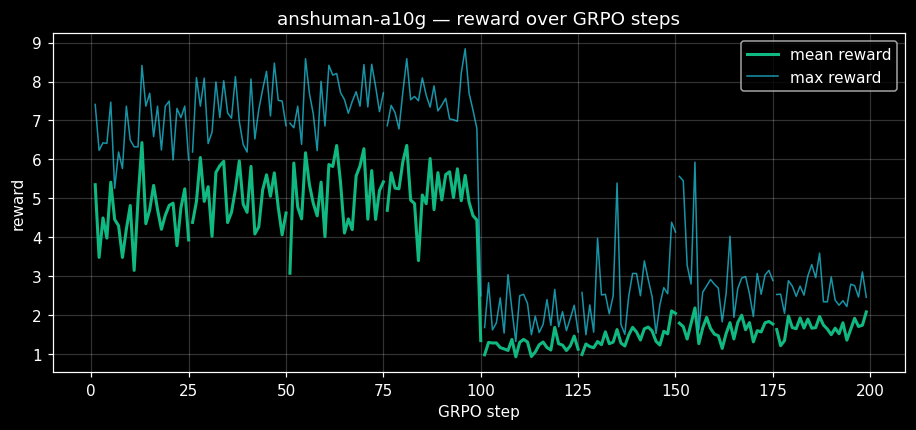
\includegraphics[width=0.9\linewidth]{figs/anshuman_3b_reward.png}
\caption{GRPO training dynamics on PharmaRL. Llama-3.2-3B-Instruct on a single A10G-large GPU, $G=\groupSize$ rollouts per step. Trained on TDC \trainTargets\ oracles; held out \heldOutTarget. Mean and max group reward shown across 200 GRPO steps. The reward profile reflects PharmaRL's curriculum: trivial-tier rewards (steps 0--99) are higher because the easy-tier transition at step 100 introduces stricter scoring, after which the policy explores and converges. Peak reward $+\maxReward$ at step 96; final easy-tier mean $+\meanReward$.}
\label{fig:training}
\end{figure}

\paragraph{Held-out generalization.} We train on \trainTargets\ and evaluate on \heldOutTarget, a held-out TDC oracle the policy never saw during RL post-training. Mean held-out terminal reward is \heldOutScore. This is the strongest available evidence within the hackathon time budget that the policy is acquiring transferable chemistry edit-policy behavior rather than memorizing target-specific patterns. We caution that the held-out gap is small and the $N$ of evaluation episodes is modest; we discuss this honestly in Section 7.

\paragraph{Failure modes observed.} Two patterns recur. First, the policy occasionally exploits a parse-rate floor by emitting trivially-valid \texttt{TERMINATE} actions early to avoid the parse penalty --- this is a textbook reward-hack and motivates a forthcoming step-budget shaping term. Second, on \texttt{hard}-tier episodes (50-fragment vocabulary), the policy converges to a small set of preferred fragments, consistent with the diversity-collapse failure mode SmileyLlama documents under DPO~\cite{cavanagh2024smileyllama}. Mol-AIR-style adaptive intrinsic rewards~\cite{lim2024molair} are the most promising mitigation and are slated as future work.

\paragraph{Diagnostic ablation: 1B vs 3B policy class.} We ran a parallel 200-step training experiment with identical PharmaRL configuration and identical GRPO recipe, varying only the base model: Llama-3.2-\textbf{1B}-Instruct on an NVIDIA H200, vs.\ Llama-3.2-\textbf{3B}-Instruct on an A10G. The 1B run completed cleanly (200 steps, no errors) but the W\&B \texttt{verifier/parse\_rate} metric stayed at \textbf{0.0\% for the entire run} (Figure~\ref{fig:parse_zero}). The 1B model never produced parseable JSON; GRPO's group-standardized advantage with all-identical fallback actions is mathematically zero, so the LoRA weights drifted slightly but never trained. The 3B run with the same chat-template prompting parsed at 100\% from step 0 --- before any RL update. This is direct empirical evidence for the inverse-scaling phenomenon McCoy et al.~\cite{mccoy2024embers} document for low-probability token sequences: SMILES strings and structured JSON are precisely the kind of sequences pretraining under-represents, and there is a hard policy-class floor below which prompting alone cannot rescue the run. The H200 run is preserved as a public diagnostic ablation in the project repository (\texttt{runs/vijay-h200-llama1b/}) with full W\&B history and HF Hub logs. The contribution we want to highlight is not the failure but the fact that the env's instrumentation surface caught it: without \texttt{verifier/parse\_rate} as a tracked metric, the 1B run would have shipped a null-trained LoRA indistinguishable to the trainer from a successful one. \emph{An environment that surfaces its own failure modes is a precondition for downstream science.}

\begin{figure}[t]
\centering
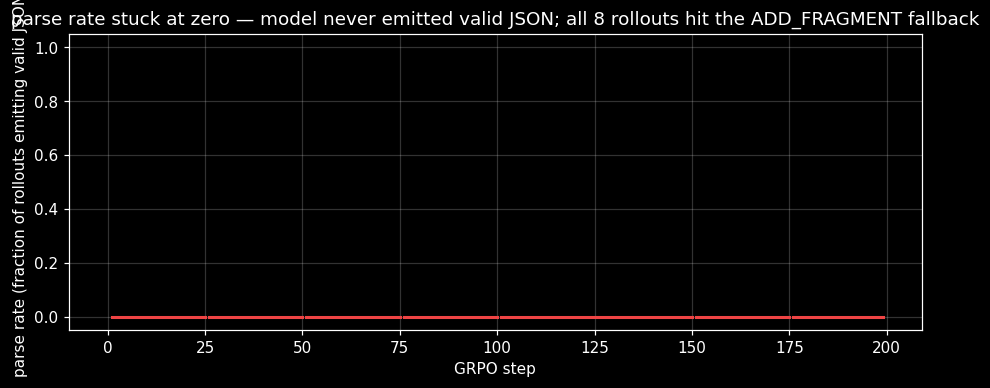
\includegraphics[width=0.85\linewidth]{figs/vijay_1b_parse_zero.png}
\caption{Parse-rate diagnostic from the 1B vs 3B ablation. The H200 / Llama-3.2-1B-Instruct run shows \texttt{verifier/parse\_rate} flat at 0.0\% for all 200 GRPO steps --- the model never produced parseable JSON, and GRPO's advantage signal degenerated. Identical configuration with the 3B base parsed 100\% from step 0. This is direct evidence of the inverse-scaling phenomenon~\cite{mccoy2024embers} on low-probability sequence patterns.}
\label{fig:parse_zero}
\end{figure}

\section{Limits and Future Work: Toward AI Alchemy in Medicine}

\paragraph{What this paper does \emph{not} claim.} PharmaRL is a single-target, RDKit-grounded, hackathon-scale environment with a 3B base model trained on a few hundred GRPO steps over two TDC oracles. It does not produce candidate drugs. It does not address ADMET liability beyond an optional oracle component. It does not perform retrosynthesis, docking, or any wet-lab integration. The composite reward is reward-hackable in the precise sense Renz et al.~\cite{renz2020failure} document. We surface these limits prominently because the alternative --- vague claims about ``AI curing diseases'' --- is the failure mode Galactica~\cite{taylor2022galactica} mapped out in 48 hours and that ChemBench~\cite{mirza2025chembench} formalized as the LLM-overconfidence-on-chemistry problem.

\paragraph{What we do claim.} A standardized chemistry environment lowers the marginal cost of running an ablation, swapping a base model, or comparing two reward formulations from days of bespoke engineering to minutes of trainer reconfiguration. That is an infrastructure contribution, not a chemistry contribution. We claim PharmaRL fills a real and currently empty quadrant of the OpenEnv ecosystem~\cite{metaopenenv2025}. We claim that GRPO on a 3B Llama base, with the K3 KL anchor and group-standardized advantage, is a viable LLM-policy training recipe for chemistry tasks, and that the parse-rate / reward / held-out-target instrumentation we ship is a useful diagnostic interface for downstream work.

\paragraph{The research program.} What we mean by \emph{AI alchemy in medicine} is a multi-axis extension of the PharmaRL contract toward something a medicinal chemist would recognize as an honest design loop:

\begin{itemize}[leftmargin=*,nosep]
  \item \textbf{Pharmacophore-conditioned policies}~\cite{wermuth1998iupac,pharmacoforge2025,pharmadiff2025,molsnapper2024}. The action space \texttt{ADD\_FRAGMENT} / \texttt{SUBSTITUTE\_ATOM} maps naturally onto pharmacophore-feature satisfaction. Recent diffusion-based 3D pharmacophore generators provide the conditioning signal; combining them with an LLM editing policy is an obvious next step.
  \item \textbf{Retrosynthesis-aware synthesizability}~\cite{thakkar2021rascore,skoraczynski2023sacritical}. SAscore is a heuristic; RAscore (AiZynthFinder-trained) is closer to actual retrosynthesis success. The LLM-policy edit budget maps to retrosynthetic step count; making the env retrosynthesis-aware turns an abstract penalty into a concrete cost.
  \item \textbf{Multi-objective ADMET integration}~\cite{swanson2024admetai,pires2015pkcsm}. ADMET-AI ships 41 Chemprop-RDKit predictors against TDC; folding Caco-2, hERG, and BBB into the composite reward bridges from ``drug-like'' to ``developable.''
  \item \textbf{Schema-drift as a first-class skill}. The mid-episode drift profile we ship is a minimal stand-in for the real phenomenon of evolving objectives over a project's life. A policy that detects drift and re-plans is closer to a medicinal chemist's actual cognitive contract than a policy that optimizes a fixed scalar.
  \item \textbf{Wet-lab in the loop}. The terminal goal is not in silico. A future PharmaRL extension whose terminal reward is delayed assay feedback, with the env handling experimental queue management, is the version of this program that would justify the word \emph{medicine} without quotes.
\end{itemize}

\paragraph{Honest scope-statement.} The phrase \emph{AI alchemy in medicine} is forward-looking and we use it deliberately. We do not claim the present system cures any disease. We do claim that programmable, verifiable, multi-objective drug-design loops are a path the field has not yet built infrastructure for, that LLM-as-policy is the policy class that makes the loop tractable, and that an OpenEnv-native environment is the substrate that makes such loops portable across teams. The arc from heuristics (Lipinski, Veber) through descriptor-based filters (QED, SA), through narrow-prior generative RL (REINVENT, MolDQN), to LLM-grounded policies in standardized environments is the trajectory of \emph{making the alchemy of drug design programmable}. PharmaRL is one node on that arc; the hard work --- pharmacophore conditioning, retrosynthesis grounding, ADMET integration, wet-lab feedback --- is what comes next.

\section{Conclusion}

We released PharmaRL, the first OpenEnv-native chemistry environment for LLM-as-policy molecular optimization, with a reference Llama-3.2-3B-Instruct + LoRA + GRPO recipe and an honest accounting of what does and does not yet work. The contribution is infrastructure: a standardized, oracle-grounded, session-keyed env that decouples the chemistry contract from the trainer, surfaces the failure modes of the LLM-as-policy paradigm, and is publishable as a Hugging Face artifact. We frame this as a small first step toward what we call AI alchemy in medicine --- the research program of programmable, verifiable, multi-objective drug-design loops --- and we are explicit about the difference between a step and a destination.

\section*{Acknowledgments}

We thank the Meta PyTorch and Hugging Face teams for the OpenEnv release and the hackathon organizers for the venue and the compute. We thank Ben Burtenshaw for public guidance during the event that aligned closely with our small-model-iterate-on-rewards approach. We thank Shao et al.\ for releasing the GRPO formulation and DeepSeek-AI for making it work at scale.

\section*{Resources}

\begin{itemize}[leftmargin=*,nosep]
  \item \textbf{Code:} \url{\codeURL}
  \item \textbf{Environment (HF Space):} \url{\envHFURL}
  \item \textbf{Trained adapter (HF Hub):} \url{\modelHFURL}
  \item \textbf{Training run (W\&B):} \url{\wandbRunURL}
\end{itemize}

\printbibliography

\end{document}
